\documentclass[oneside,14pt]{book}

\usepackage[T1,T2A]{fontenc}
\usepackage[utf8]{inputenc}
\usepackage[english,russian]{babel}
\usepackage{indentfirst}

%\usepackage[paperwidth=15cm,paperheight=7.5cm]{geometry} % планшет
%\usepackage[paperwidth=297mm,paperheight=210mm]{geometry} % A4
%\usepackage[paperwidth=148mm,paperheight=105mm]{geometry} % A5
\usepackage[paperwidth=18cm,paperheight=13cm,margin=5mm]{geometry} % экран*2

%\usepackage[colorlinks=true,
%]{hyperref}
%\newcommand{\email}[2]{#1\ \href{mailto:#2}{<\nolinkurl{#2}>}}
% %\newcommand{\email}[2]{\emph{#1\ <#2>}}
\usepackage[unicode,colorlinks,
pdftitle={Azbuka ARMaturschika (ru)},
pdfauthor={(c) Dmitry Ponyatov <dponyatov@gmail.com>, SSAU ASCL},
pdfsubject={ru manual on writing programs for Cortex-M MCUs},
pdfkeywords={ARM} {Cortex} {MCU} {ARMatura} {Arduino} {SSAU}
]{hyperref}

\usepackage{wrapfig}
\usepackage{graphicx}
\usepackage{epstopdf}
\DeclareGraphicsExtensions{.eps}

\usepackage{listings}
\usepackage{dirtree}
\usepackage[usenames,dvipsnames,svgnames]{xcolor}
\newcommand{\cppcolor}{\color[rgb]{0.94, 0.97, 1.0}} % Alice blue
\newcommand{\asmcolor}{\color[rgb]{0.98, 0.92, 0.84}} % Antique white
\newcommand{\ldcolor}{\color[rgb]{0.67, 0.9, 0.93}} % Blizzard Blue
\newcommand{\concolor}{\color[rgb]{0.88, 1.0, 1.0}} % Light cyan
\newcommand{\makecolor}{\color[rgb]{0.9, 0.9, 0.98}} % Lavender mist

%\definecolor{cppcolor}{rgb}{0.94, 0.97, 1.0}
\lstset{frame=single,
numbers=left, numberstyle=\small, numbersep=1mm,
tabsize=4,
keywordstyle=\color{blue}\texttt,
commentstyle=\color{cyan}\texttt,
inputencoding=utf8, extendedchars=true, showspaces=false,  
inputencoding=cp1251
}
\usepackage{lstlangarm}
\usepackage{lstlanggnumake}
\usepackage{lstlanggnuld}
\usepackage{lstlanggnudump}

\lstdefinestyle{cpp}{language=C++,backgroundcolor=\cppcolor}
\lstdefinestyle{asm}{language={[ARM]Assembler},backgroundcolor=\asmcolor}
\lstdefinestyle{gnuld}{language={[GNU]Link},backgroundcolor=\ldcolor}
\lstdefinestyle{con}{backgroundcolor=\concolor}
\lstdefinestyle{mk}{language=[GNU]Make,backgroundcolor=\makecolor}
\lstdefinestyle{objdump}{language=[GNU]Dump}

\newcommand{\cm}[1]{Cortex-M#1}
\newcommand{\cx}{\cm{x}}

\newcommand{\vld}{STM32VLDISCOVERY}

%\renewcommand{\url}[1]{\textbf{#1}}
\newcommand{\email}[1]{$<$\href{mailto:#1}{\textbf{#1}}$>$}

\newcommand{\cpp}{$C^{+^{+}}$}

\newcommand{\cp}[1]{\footnote{копипаста: #1}}

\newcommand{\thmod}{Thumb}
\newcommand{\armod}{ARM}
\newcommand{\arm}{ARM}

\newcommand{\Reg}[1]{\textbf{#1}}
\newcommand{\R}[1]{\Reg{R#1}}

\newcommand{\periph}[1]{\texttt{#1}}
\newcommand{\jtag}{\periph{JTAG}}

\usepackage{wasysym} % smileys
\usepackage{gensymb} % celsius
\usepackage{amssymb} % windows key
\usepackage{textcomp} % bigcircle

\usepackage[os=win]{menukeys}
\newcommand{\winstart}{$\boxplus$}
\newcommand{\file}[1]{\textbf{\textsf{#1}}}
\newcommand{\window}[1]{\textbf{\textit{#1}}}
\newcommand{\alarm}[1]{{\color{DarkRed}#1}}
\newcommand{\wcmd}[1]{\keys{\winstart+R}\ \directory{#1}}
\newcommand{\checkbox}{$\boxtimes$}
\newcommand{\uncheckbox}{$\square$}
\newcommand{\lms}{\keys{$\lhd$}}
\newcommand{\rms}{\keys{$\rhd$}}
\newcommand{\eclpx}{\window{Project Explorer}}

\newcommand{\win}[1]{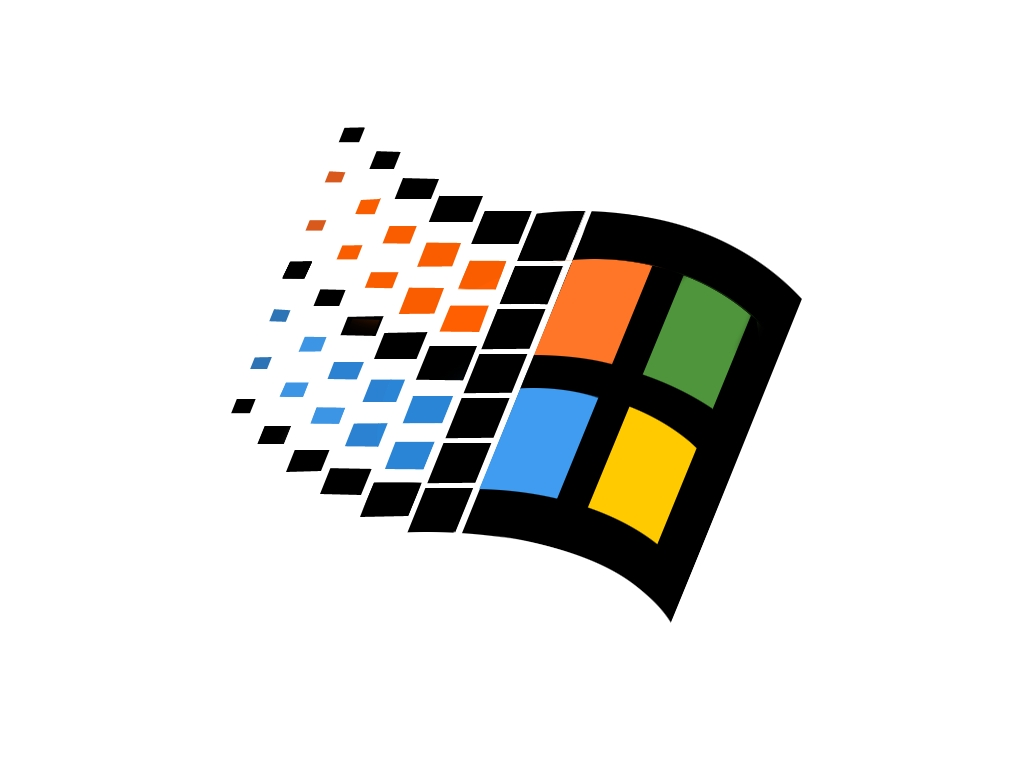
\includegraphics[height=10ex]{fig/winlogo.jpg} #1}
\newcommand{\lin}[1]{
\includegraphics[height=10ex]{fig/linuxcolor.png} #1}
\newcommand{\bug}{
\includegraphics[height=10ex]{fig/iconbug.png}}

\newcommand{\linux}{Linux}
\newcommand{\git}{Git}
\newcommand{\eclipse}{\textcircled{$\equiv$}\textsc{eclipse}}
%\newcommand{\term}[1]{\underline{#1}}
\newcommand{\term}[1]{\underline{\color{DarkBlue} #1}}
\newcommand{\miktex}{MiK\TeX}
\newcommand{\internet}{Internet}
\newcommand{\ql}{Quantum$^{\circledR}L^{e}aPs$}
\newcommand{\gdb}{GDB}

\newcommand{\make}{\file{make}}
\newcommand{\makefile}{\file{Makefile}}

\usepackage{tocloft}
\newcommand{\listlabname}{Лабораторные работы}
\newlistof{lab}{ex}{\listlabname}
\newcommand{\labpart}[1]{\addcontentsline{ex}{part}{#1}}
\newcounter{labworkcounter}
\newcommand{\labwork}[1]{
\refstepcounter{labworkcounter}
\section*{ЛР\thelabworkcounter: #1}
\addcontentsline{toc}{subsection}{ЛР\thelabworkcounter: #1}
\addcontentsline{ex}{section}{ЛР\thelabworkcounter: #1}
}
\newcommand{\labref}[1]{ЛР\ref{#1}}

\newcommand{\thetitle}{Азбука халтурщика-ARMатурщика}

\newcommand{\mytitle}[1]{
\title{\Huge{\thetitle}\\
#1\\
\normalsize{учебный курс по микроконтроллерам \cx:\\
Миландр 1986ВЕ, STM32F, LPC21xx}}
}

\author{(copypasta) Понятов Д.А. \email{dponyatov@gmail.com}, ИКП СГАУ}


\begin{document}

%\title{\Huge{Азбука ARMатурщика}\\
%\normalsize{учебный курс по микроконтроллерам \cx:\\
%Миландр 1986ВЕ, STM32F, LPC21xx}}
%\author{\copyright\\
%Понятов Д.А. \email{dponyatov@gmail.com}, ИКП СГАУ, \\
%Недяк С.П. \email{fvs@fet.tusur.ru}, ТУСУР
%}
%\maketitle
%\tableofcontents
%\listoflab
%
%\part{Обзор семейства микроконтроллеров \cx}
%
%\chapter{Архитектура ARM}

\cp{\url{http://ru.wikipedia.org/wiki/ARM}} %\_(архитектура)

Архитектура ARM (Advanced RISC Machine, Acorn RISC Machine, 
усовершенствованная RISC-машина)\ --- семейство лицензируемых 32-битных и 
64-битных микропроцессорных ядер разработки компании ARM Limited.

Среди лицензиатов: практически все заметные разработчики цифровых
электронных компонентов.
Многие лицензиаты делают собственные версии ядер на базе ARM.

Значимые семейства процессоров: ARM7, ARM9, ARM11 и Cortex.

В 2007 году около 98\% из более чем миллиарда мобильных телефонов, продаваемых 
ежегодно, были оснащены по крайней мере одним процессором ARM. По состоянию 
на 2009 на процессоры ARM приходилось до 90\% всех встроенных 32-разрядных 
процессоров. Процессоры ARM широко используются в потребительской 
электронике\ --- в том числе КПК, мобильных телефонах, цифровых носителях и 
плеерах, портативных игровых консолях, калькуляторах и компьютерных п
ериферийных устройствах, таких как жесткие диски или маршрутизаторы.

Эти процессоры имеют низкое энергопотребление, поэтому находят широкое 
применение во встраиваемых системах и преобладают на рынке мобильных 
устройств, для которых данный фактор немаловажен.

В настоящее время значимыми являются несколько семейств процессоров ARM:

\begin{itemize}
\item ARM7 (с тактовой частотой до 60-72 МГц), предназначенные, например, для 
недорогих мобильных телефонов и встраиваемых решений средней производительности. 
В настоящее время активно вытесняется новым семейством Cortex.
\item ARM9, ARM11 (с частотами до 1 ГГц) для продвинутых телефонов, карманных 
компьютеров и встраиваемых решений высокой производительности.
\item Cortex A\ --- новое семейство процессоров на смену ARM9 и ARM11.
\item Cortex M\ --- новое семейство процессоров на смену ARM7, также 
призванное занять новую для ARM нишу встраиваемых решений низкой 
производительности. В семействе присутствуют три значимых ядра: \cm{0}, 
\cm{3} и \cm{4}.
\end{itemize}

\paragraph{Архитектура}

Существует спецификация архитектуры ARM Cortex, которая разграничивает все типы опций, 
которые поддерживает ARM, так как детали реализации каждого типа процессора м
огут отличаться. Архитектура развивалась с течением времени, и начиная с 
ARMv7 были определены 3 профиля:
\begin{itemize}
\item{A (application)} для устройств, требующих высокой производительности (смартфоны, планшеты)
\item{R (real time)} для приложений, работающих в реальном времени,
\item{M (microcontroller)} для микроконтроллеров и недорогих встраиваемых устройств.
\end{itemize}

\paragraph{Режимы процессора}

Процессор может находиться в одном из следующих рабочих режимов:
\begin{itemize}
\item{User mode} — обычный режим выполнения программ. В этом режиме 
выполняется большинство программ.
\item{Fast Interrupt (FIQ)} — режим быстрого прерывания (меньшее время с
рабатывания)
\item{Interrupt (IRQ)} — основной режим прерывания.
\item{System mode} — защищённый режим для использования операционной системой.
\item{Abort mode} — режим, в который процессор переходит при возникновении 
ошибки доступа к памяти (доступ к данным или к инструкции на этапе 
prefetch конвейера).
\item{Supervisor mode} — привилегированный пользовательский режим.
\item{Undefined mode} — режим, в который процессор входит при попытке 
выполнить неизвестную ему инструкцию.
\end{itemize}

Переключение режима процессора происходит при возникновении соответствующего 
исключения, или же модификацией регистра статуса.

\paragraph{Набор команд ARM}

Режим, в котором исполняется 32-битный набор команд.

\paragraph{Набор команд \thmod}

Для улучшения плотности кода процессоры, начиная с ARM7TDMI, снабжены режимом 
\thmod. В этом режиме процессор выполняет альтернативный набор 16-битных 
команд. Большинство из этих 16-разрядных команд переводятся в нормальные 
команды ARM. Уменьшение длины команды достигается за счет сокрытия некоторых 
операндов и ограничения возможностей адресации по сравнению с режимом полного 
набора команд ARM.

В режиме \thmod\ меньшие коды операций обладают меньшей функциональностью. 
Например, только ветвления могут быть условными, и многие коды операций имеют 
ограничение на доступ только к половине главных регистров процессора. Более 
короткие коды операций в целом дают большую плотность кода, хотя некоторые 
операции требуют дополнительных команд. В ситуациях, когда порт памяти или 
ширина шины ограничены 16 битами, более короткие коды операций режима 
\thmod\ становятся гораздо производительнее по сравнению с обычным 32-битным ARM 
кодом, так как меньший программный код придется загружать в процессор при 
ограниченной пропускной способности памяти.

Аппаратные средства типа Game Boy Advance, как правило, имеют небольшой объём 
оперативной памяти доступной с полным 32-битным информационным каналом. Но 
большинство операций выполняется через 16-битный или более узкий информационный 
канал. В этом случае имеет смысл использовать \thmod\ код и вручную 
оптимизировать некоторые тяжелые участки кода, используя переключение в 
режим \armod.

\paragraph{Набор команд \thmod2}

\thmod2 — технология, стартовавшая с ARM1156 core, анонсированного в 2003 
году. Он расширяет ограниченный 16-битный набор команд Thumb дополнительными 
32-битными командами, чтобы задать набору команд дополнительную ширину. Цель 
\thmod2\ --- достичь плотности кода как у Thumb, и производительности как у 
набора команд \armod\ на 32 битах. Можно сказать, что в ARMv7 эта цель была 
достигнута.

\thmod2 расширяет как команды \armod, так и команды \thmod\ ещё большим 
количеством команд, включая управление битовым полем, табличное ветвление, 
условное исполнение. Новый язык «Unified Assembly Language» (UAL) поддерживает 
создание команд как для ARM, так и для Thumb из одного и того же исходного 
кода. Версии \thmod\ на ARMv7 выглядят как код ARM. Это требует осторожности и 
использования новой команды if-then, которая поддерживает исполнение до 4 
последовательных команд испытываемого состояния. Во время компиляции в ARM 
код она игнорируется, но во время компиляции в код \thmod2 генерирует команды.

\paragraph{Набор команд Jazelle}

Jazelle — это технология, которая позволяет байткоду Java исполняться прямо 
в архитектуре ARM в качестве 3-го состояния исполнения (и набора команд) 
наряду с обычными командами ARM и режимом Thumb. Поддержка технологии Jazelle 
обозначается буквой «J» в названии процессора — например, ARMv5TEJ. Данная 
технология поддерживается начиная с архитектуры ARMv6, хотя новые ядра 
содержат лишь ограниченные реализации, которые не поддерживают аппаратного 
ускорения.

\paragraph{ARMv8 и набор команд ARM 64 бит}

В конце 2011 года была опубликована новая версия архитектуры, ARMv8. В ней 
появилось определение архитектуры AArch64, в которой исполняется 64-битный 
набор команд A64. Поддержка 32-битных команд получила название A32 и
 исполняется на архитектурах AArch32. Инструкции Thumb поддерживаются в 
 режиме T32, только при использовании 32-битных архитектур. Допускается 
 исполнение 32-битных приложений в 64-битной ОС, и запуск виртуализованной 
 32-битной ОС при помощи 64-битного гипервизора.[47] Applied Micro, AMD, 
 Broadcom, Calxeda, HiSilicon, Samsung, STM и другие заявили о планах по 
 использованию ARMv8. Ядра Cortex-A53 и Cortex-A57, поддерживающие ARMv8, 
 были представлены компанией ARM 30 октября 2012 года.[48]

Как AArch32, так и AArch64, поддерживают VFPv3, VFPv4 и advanced SIMD (NEON). 
Также добавлены криптографические инструкции для работы с AES, SHA-1 и SHA-256.

\paragraph{Условное исполнение}

Одним из существенных отличий архитектуры ARM от других архитектур ЦПУ 
является так называемая предикация — возможность условного исполнения команд. 
Под «условным исполнением» здесь понимается то, что команда будет выполнена 
или проигнорирована в зависимости от текущего состояния флагов состояния 
процессора.

В то время как для других архитектур таким свойством, как правило, обладают 
только команды условных переходов, в архитектуру ARM была заложена 
возможность условного исполнения практически любой команды. Это было 
достигнуто добавлением в коды их инструкций особого 4-битового поля 
(предиката). Одно из его значений зарезервировано на то, что инструкция 
должна быть выполнена безусловно, а остальные кодируют то или иное сочетание 
условий (флагов). С одной стороны, с учётом ограниченности общей длины 
инструкции, это сократило число бит, доступных для кодирования смещения в 
командах обращения к памяти, но с другой — позволило избавляться от 
инструкций ветвления при генерации кода для небольших if-блоков.

Пример, обычно рассматриваемый для иллюстрации — основанный на вычитании 
алгоритм Евклида. В языке C он выглядит так:

\begin{lstlisting}[style=cpp,title={алгоритм Евклида}]
while (i != j) {
       if (i > j)
           i -= j;
       else
           j -= i;
}
\end{lstlisting}

А на ассемблере ARM — так:

\begin{lstlisting}[style=asm]
loop CMP Ri, Rj; set condition "NE" if (i != j),
						; "GT" if (i > j),
						; or "LT" if (i < j)
	SUBGT  Ri, Ri, Rj   ; if "GT" (greater than), i = i-j;
	SUBLT  Rj, Rj, Ri   ; if "LT" (less than), j = j-i;
	BNE    loop         ; if "NE" (not equal), then loop
\end{lstlisting}

Из кода видно, что использование предикации позволило полностью избежать 
ветвления в операторах else и then. Заметим, что если Ri и Rj равны, то ни 
одна из SUB инструкций не будет выполнена, полностью убирая необходимость в 
ветке, реализующей проверку while при каждом начале цикла, что могло быть 
реализовано, например, при помощи инструкции SUBLE (меньше либо равно).

Один из способов, которым уплотнённый (Thumb) код достигает большей экономии 
объёма — это именно удаление 4-битового предиката из всех инструкций, кроме 
ветвлений.

\paragraph{Другие особенности}

Другая особенность набора команд это возможность соединять сдвиги и вращения 
в инструкции «обработки информации» (арифметическую, логическую, движение 
регистр-регистр) так, что, например выражение С:
\begin{lstlisting}[style=cpp]
a += (j << 2);
\end{lstlisting}

может быть преобразовано в команду из одного слова и одного цикла в ARM:

\begin{lstlisting}[style=asm]
ADD Ra, Ra, Rj, LSL #2
\end{lstlisting}

Это приводит к тому, что типичные программы ARM становятся плотнее, чем 
обычно, с меньшим доступом к памяти. Таким образом, конвейер используется 
гораздо более эффективно. Даже несмотря на то, что ARM работает на скоростях, 
которые многие бы сочли низкими, он довольно-таки легко конкурирует с 
многими более сложными архитектурами ЦПУ.

ARM процессор также имеет некоторые особенности, редко встречающиеся в 
других архитектурах RISC — такие, как адресация относительно счетчика 
команд (на самом деле счетчик команд ARM является одним из 16 регистров), 
а также пре- и пост-инкрементные режимы адресации.

Другая особенность, которую стоит отметить, это то, что некоторые ранние 
ARM процессоры (до ARM7TDMI), например, не имеют команд для хранения 
2-байтных чисел. Таким образом, строго говоря, для них невозможно 
сгенерировать эффективный код, который бы вел себя так, как ожидается от 
объектов С, типа \verb|volatile int16_t|.


%
%\section{\cx}
%\chapter{Периферия}
%\section{Таймеры}
%\section{DMA}
%\section{UART}
%\section{CAN}
%\section{USB}
%\section{Ethernet}
%\chapter{Производители}
%\section{ST Microelectronics}
%\subsection{STM32F0xx /\cm{0}/}
%\subsection{STM32F1xx} \cm{1} VLDISCOVERY
\url{www.st.com/stm32-discovery}

%\subsection{STM32F4xx /\cm{4}/} STM32F4DISCOVERY
%
%\secru{ЗАО <<ПКК Миландр>>}\secdown

Компания <<Миландр>> выпускает МК для спецприменений,
и (относительно) дешевые варианты МК в пластиковом корпусе для обучения
и неответственных применений.

\bigskip

\begin{tabular}{l l}
Телефон:& (495) 981-54-33 (8.30-17.00, отдел маркетинга и продаж *)\\
Факс:& (495) 981-54-36\\
E-mail:& \email{info@milandr.ru}\\
Сайт:& \url{http://www.milandr.ru}\\
Форум:& \url{http://forum.milandr.ru}\\
Адрес:& 124498, г. Москва, Зеленоград, проезд 4806, дом 6\\
\end{tabular}

\secru{КР1986ВЕ9х /\cm{3}/}

\begin{wrapfigure}{r}{0.3\textwidth}
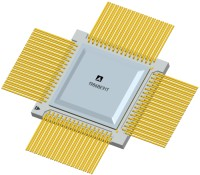
\includegraphics[width=0.3\textwidth]{fig/1986BE94.jpg}
\end{wrapfigure}

\bigskip
\begin{tabular}{l l}
Аналог & STM32F103x\ref{stm32f1}\\
ROM (Flash) & 128K \\
RAM & 32K \\
VCC & $2.2\div3.6$ V\\
Freq & 80 MHz \\
$T^o$ & $-60\div+125$\celsius \\
USB & client/host (12 MBit/s) \\
UART & 2\\
CAN & 2\\
ADC & 2x 12bit 1msps\\
DAC & 12bit\\
\end{tabular}

\bigskip

\begin{tabular}{l l l l l l l l l}
& Pins & SPI & $I^{2}C$ & ADC & DAC & CMP & extBUS &исполнение \\
\hline
1986ВЕ91Т &96 &2 &1 &16ch &2 &3 &32bit &ПЗ5,QFP\\
1986ВЕ94Т &96 &2 &1 &16ch &2 &3 &32bit &ПЗ5\\
1986ВЕ92У  &43 &2 &1 &8ch  &1 &2 &8bit &ПЗ5\\
MDR32F9Q2I &   &  &  &     &  &  &     &QFP\\
К1986ВЕ92QI &   &  &  &     &  &  &     &QFP\\
1986ВЕ93Т &30 &1 &  &4ch  &1 &2 & &ПЗ5\\
\end{tabular}

\secru{1986ВЕ4У /\cm{0}/}

32-разрядный RISC-микроконтроллер с 8-канальным 24-разрядным $\Sigma\Delta$ АЦП

\bigskip
\begin{tabular}{l l}
ROM (Flash) & 128K \\
RAM & 16K \\
VCC & $2.2\div3.6$ V\\
Freq & 36 MHz \\
$T^o$ & $-60\div+125$\celsius, К $0\div 70$\celsius\\
UART & 2\\
ADC & $\Sigma\Delta$ 24bit, 12bit \\
DAC & 12bit\\
\end{tabular}

\bigskip

\begin{tabular}{l l l l l l l l l}
& Pins & SPI & $I^{2}C$ & ADC & DAC & CMP & extBUS &исполнение \\
\hline
1986ВЕ4У &36 &1 & &8/8ch &1 & & &ПЗ5 \\
\end{tabular}

\secru{1986ВЕ1Т, К1986ВЕ1QI}

\secup

%
%\section{NXP}
%\subsection{LPC210x}

\part{Программное обеспечение}
\chapter{Рабочая среда разработчика встраиваемых систем}


\begin{itemize}
  \item Операционная система с набором типовых утилит
  
  Для Windows требуется дополнительно установить несколько модулей из пакета
  \file{GnuWin32}, чтобы обеспечить минимальную совместимость с UNIX-средой.
  Установка \file{GnuWin32}\ описана в \labref{winsoftinstall}.
  
  Установка Linux описана в \labref{debianinstall}.
  
  \item Система управления версиями (\term{VCS})
  
  VCS предназначены для хранения полной истории изменений файлов проекта, и
  позволяют получить выгрузку проекта на любой момент времени, вести несколько
  веток разработки, получить историю изменений конкретного файла, или сравнить
  две версии файла (\term{diff}).
  
  Установка VCS \git\ описана в \labref{gitinstall}.
  
  \item Текстовый редактор или интегрированная среда разработки (IDE)
  
  Редактирование текстов программ и скриптов сборки (компиляции) с
  цветовой подсветкой синтаксиса (в зависимости от языка файла),
  \term{автодополнением}\ и вызовом программ-утилит нажатием сочетаний 
  клавиш. Также включает различные вспомогательные функции, например
  отладочный интерфейс и отображение объектов программ.
  
  Установка IDE \eclipse\ описана в \labref{eclipseinstall}.
  
  \item Тулчайн
  
  Пакет кросс-компилятора, ассемблера, линкера и других утилит типа make,
  objdump,.. для получения прошивок из исходных текстов программ.
  
  Установка GNU toolchain описана в \labref{gnuinstall}.
  
  \item ПО для программатора, JTAG-адаптера
  
  Загрузка полученной прошивки в целевое устройство, редактирование памяти, 
  внутрисхемная отладка в процессе работы устройства, прямое измение сигналов на
  выводах процессора (граничное сканирование и тестирование железа).
  
  Установка ПО для адаптеров ST-Link \labref{stlinkinst}, Segger J-Link
  \labref{jlinkinst}.
  
  \item Симулятор для отладки программ без железа
  
  Симулятор может использоваться как ограниченная замена реального железа
  для начального обучения, и для отладки программ, не завязанных на работу
  железа.
  
  Установка QEMU \labref{qemuinstall}.
  
  \item Система верстки документации
  
  Для документирования проектов и написания руководств нужна система верстки
  документации, выполняющая трансляцию текстов программ и файлов 
  документации в выходной формат, чаще всего \file{.pdf} и \file{.html}.
  
  Установка \LaTeX\ \labref{texinstall}.
  
\end{itemize}



\labpart{Установка ПО}

\section{Выбор и установка операционной системы}

\subsection{MacOS}

Этот странный пока случай не рассматриваем\ --- у меня нет под рукой Мака \smiley.

\subsection{Windows}

Самый распространенный вариант. Вам придется ограничиться этим вариантом если вам не повезло
с поставщиком контроллера: windows-only ПО поддержки, например софт для программатора, или
внезапно библиотеки только для коммерческих компиляторов. Аналогичная ситуация будет в случае
покупки какого-нибудь специфичного оборудования (лог.анализатор, измерительное 
оборудование или просто принтер).

Установку ОС не рассматриваем.

\win{Секции текста книги, зависящие от ОС, будут выделены вот так.}

Для разработки встраиваемого ПО нужно поставить несколько пакетов, обеспечивающих
совместимость с UNIX средами \ref{winsoftinstall}.

\subsection{Linux}\label{linux}

\begin{enumerate}
\item \label{linuxref1}\linux\ удобен для разработчика, 
\item Если он вам не удобен, см п.\ref{linuxref1}
\end{enumerate}

\lin{Секции текста книги, зависящие от ОС, будут выделены вот так.}

\lin{\labwork{Установка Debian GNU/Linux}\label{debianinstall}}

\section{Установка инструментального программного обеспечения}

\win{\labwork{Установка инструментального ПО для Windows}\label{winsoftinstall}}

Создадим рабочий каталог, установим систему контроля версий \git\ref{git}\ и 
получим локальную копию проекта этой книги, содержащий кроме текста для издательской системы
\LaTeX\ еще и исходные коды библиотек, примеры кода и т.п., которые вы захотите
использовать в своих проектах.

%\labsection{Установка Git}\label{gitinstall}

\bigskip\wcmd{\url{http://git-scm.com/download/win}}

Запуститься закачка установочного пакета scm-git (\file{Git-1.9.4-preview20140611.exe}), после его загрузки
запустите установщик, 

\bigskip
\menu{Welcome>Next}

\bigskip
\menu{GNU GPL>Next} 

\bigskip
\menu{Select components>Windows Explorer Integration>Simple Context Menu>Git GUI here>Next}

\bigskip
\menu{Use Git and optional Unix tools from the Command Prompt>Next}

\bigskip
\menu{Use OpenSSH>Next}

\bigskip
\menu{Checkout Windows-style>Next}

\bigskip
\menu{Extracting files...}

\bigskip
\menu{Completing Setup>\uncheckbox\ View ReleaseNotes>Finish}

\bigskip
Проверим что \git\ правильно установился:

\bigskip\wcmd{cmd}

\bigskip
\begin{lstlisting}[style=con]
C:\Documents and Settings\pda>git --version
git version 1.9.4.msysgit.0
\end{lstlisting}

\bigskip
Первое, что вам следует сделать после установки \git а\ ---указать ваше имя и
адрес электронной почты. Это важно, потому что каждый коммит в \git е содержит
эту информацию, и она включена в коммиты, передаваемые вами:
\begin{lstlisting}[style=con]
C:\Documents and Settings\pda>git config --global user.name "Vasya Pupkin"
C:\Documents and Settings\pda>git config --global user.email no@mail.com
C:\Documents and Settings\pda>git config --global push.default simple
\end{lstlisting}

\bigskip
Эти настройки достаточно сделать только один раз, поскольку в этом случае 
\git\ будет использовать эти данные для всего, что вы делаете.
 Если для каких-то отдельных проектов вы хотите указать другое имя или
электронную почту, можно выполнить эту же команду без параметра \verb|--global|
в каталоге с нужным проектом.

\bigskip
Создаем каталог \directory{D:/ARM}\ и выгружаем текущую копию этой книги из репозитория
\url{https://github.com/ponyatov/CortexMx}

\bigskip\wcmd{cmd}

\bigskip
\begin{lstlisting}[style=con]
C:\Documents and Settings\ponyatov>D:
D:\>mkdir \ARM
D:\>cd \ARM
D:\ARM>git clone --depth=1 https://github.com/ponyatov/CortexMx.git book
\end{lstlisting}



\lin{\labwork{Установка инструментального ПО для \linux}\label{linsoftinstall}}

\chapter{Управление версиями при написании ПО}

\section{Git}\label{git}\cite{progit}


%\chapter{Eclipse / GNU toolchain}
%\section{Утилита Make}
%\section{binutils}
%\subsection{Ассемблер GNU AS}
%\subsection{Линкер LD}
%\subsection{Утилиты работа с файлами форма та ELF}
%\section{Компилятор GCC}
%\section{IDE Eclipse}
%\chapter{Keil MDK-ARM}
%\chapter{IAR Embeded Workbench}
%
%Великолепный вводный видеокурс по IAR и основам разработки на ARM
%
%\menu{\cite{quantumleaps}>QuickStart>\href{http://youtu.be/3V9eqvkMzHA}{Lesson 0: Getting Started}}
%
%\part{Встраиваемый \cpp}
%
%\part{RTOS}
%\chapter{FreeRTOS}
%\chapter{Keil RTX}
%
%\part{Автоматное программирование /фреймворк QuantumLeaps/}

\addcontentsline{toc}{part}{Литература}
\begin{thebibliography}{9}

\bibitem{leaps}{\copyright\ Quantum Leaps}

\bibitem{milandr}{\url{http://milandr.ru/} ЗАО <<ПКК Миландр>>}

\bibitem{progit}{\url{http://git-scm.com/book/ru} перевод:
Scott Chacon
\textbf{Pro Git}
}

\bibitem{habraQP}{\url{http://habrahabr.ru/post/114239/} хабра: Quantum Leaps QP
и диаграммы состояний в UML}

\bibitem{quantumleaps}{\url{http://www.state-machine.com/}
Quantum$^{\circledR}L^{e}aPs$ State Machines \& Tools}

\end{thebibliography}


\end{document}
